\section{Motivations}

The author claims that domination of NLP by neural network models is hampered \textbf{\textit{only}} by:
\begin{enumerate}
  \item \textit{their limited ability to generalize}
  \item \textit{questionable sample complexity}:
    \begin{enumerate}
      \item their poor grasp of grammar
      \item their inability to chunk input sequences into meaningful units. While
      direct attacks on the latter are possible,
    \end{enumerate}
\end{enumerate}

In this work, authors chose a natural language-agnostic approach to improve
the generalization ablity of LSTM rather than directly attack the later since
they believe the innovatioins in RNN architecture tend to have a trickle-down
effect from language modeling to many other tasks.

While the LSTM is typically presented as a solution to the vanishing gradients
problem, its gate $i$ can also be interpreted as scaling the rows of weight matrices
$W^{j\text{*}}$ (ignoring the non-linearity in $j$).

\section{Model}

The standard LSTM update is a function:

$$\text{LSTM}(\boldsymbol{x}, \boldsymbol{c}_{\text{prev}}, \boldsymbol{h}_{\text{prev}}):
\mathbb{R}^m \times \mathbb{R}^n \times \mathbb{R}^n \rightarrow \mathbb{R}^n \times \mathbb{R}^n$$
$$\text{LSTM}(\boldsymbol{x}, \boldsymbol{c}_{\text{prev}}, \boldsymbol{h}_{\text{prev}})
= (\boldsymbol{c}, \boldsymbol{h})$$.

Before the standard LSTM update taking place, a mogrifier is used. The mogrifier
is essentially a gate prior to the input into each LSTM cell, and it is entirely
based on the interaction between the hidden state and the input. In the mogrifier,
$\boldsymbol{x}$ and $\boldsymbol{h}_{\text{prev}}$ modulate one another in an alternating
fashion. See Figure \ref{fig1} for this process.

\begin{figure}[ht]
  \centering
  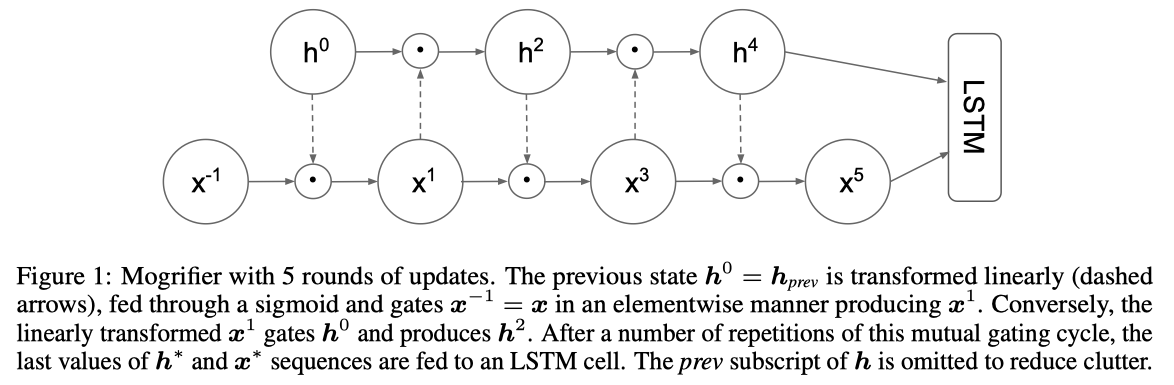
\includegraphics[scale=0.4]{images/MogrifierLSTM.png}
  \caption{Mogrifier LSTM.}
  \label{fig1}
\end{figure}

Mogrifier($\boldsymbol{x}, \boldsymbol{c}_{\text{prev}}, \boldsymbol{h}_{\text{prev}}$) =
LSTM($\boldsymbol{x}^\uparrow, \boldsymbol{c}_{\text{prev}}^{\uparrow}, \boldsymbol{h}_{\text{prev}}^{\uparrow}$).
$\boldsymbol{x}^\uparrow$ and $\boldsymbol{h}_{\text{prev}}^{\uparrow}$ are
defined as the highest indexed $x^i$ and $\boldsymbol{h}^{i}_{\text{prev}}$ as
in equation(\ref{eq1}) and (\ref{eq2}), where $\boldsymbol{x}^{-1} = \boldsymbol{x}$
and $\boldsymbol{h}_{\text{prev}}^{0} = \boldsymbol{h}_{\text{prev}}$, $r \in \mathbb{R}$
is a hyperparameter. $r = 0$ recovers LSTM.

\begin{eqnarray}
%\begin{aligned}
\boldsymbol{x}^i &= 2\sigma(\boldsymbol{Q}^i\boldsymbol{h}_{\text{prev}}^{i-1})
\odot \boldsymbol{x}^{i-2}, \qquad \text{for odd  } i \in [1\dotsc r] \label{eq1}\\
\boldsymbol{h}^i_{\text{prev}} &= 2\sigma(\boldsymbol{R}^i\boldsymbol{x}^{i-1})
\odot \boldsymbol{h}^{i-2}_{\text{prev}}, \qquad \text{for even  } i \in [1\dotsc r] \label{eq2}
%\end{aligned}
\end{eqnarray}

\section{Compare with other RNNs}

Input Switched Affine Network \cite{foerster2017input};
Hypernetworks \cite{ha2016hypernetworks};
Multiplicative LSTM\cite{krause2016multiplicative};
